\documentclass[11pt]{article}
\usepackage{geometry}
\geometry{a4paper}

\usepackage{graphicx}
\usepackage{amsmath,amsthm,amssymb}
\usepackage{amsfonts}
\usepackage{eucal}
\usepackage{gensymb}
\usepackage{yfonts}
\usepackage{epic}
\usepackage{verbatim}
\usepackage{xcolor}
\usepackage{enumitem}
\usepackage{hyperref}
\usepackage{cleveref}
\hypersetup{colorlinks=true,citecolor=blue,linkcolor=blue}
\usepackage{textcomp}
\usepackage{marginnote}
\usepackage{color}

\usepackage{fancyhdr}
\usepackage{float}
\usepackage{mdframed}

\usepackage{wrapfig}

\mdfsetup{nobreak=true}

\oddsidemargin=.2in
\evensidemargin=.2in
\topmargin=-.5in
\textheight=8.5in
\textwidth=6in

\usepackage{mathtools}
\DeclarePairedDelimiter{\ceil}{\lceil}{\rceil}
\DeclarePairedDelimiter{\floor}{\lfloor}{\rfloor}

\renewcommand{\headrulewidth}{0.2pt}
\newcommand{\N}{\mathbb{N}}
\newcommand{\Z}{\mathbb{Z}}
\newcommand{\Q}{\mathbb{Q}}
\newcommand{\R}{\mathbb{R}}
\newcommand{\C}{\mathbb{C}}
\newcommand{\p}{\mathcal{P}}
\newcommand{\h}{\mathcal{H}}

\renewcommand{\epsilon}{\varepsilon}

\newcommand*\sierpinski{\vcenter{\hbox{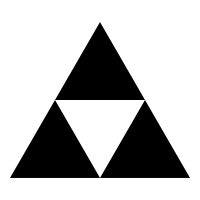
\includegraphics[width=1em]{SierpinskiTriangleIcon.png}}}}

\newcommand{\teamno}{213}

\begin{document}
\thispagestyle{empty}
\noindent \huge{Team Number:} \underline{\teamno\phantom{}}

\vspace{.5cm}
\noindent \huge{PUMaC 2024 Power Round Cover Sheet}

\vspace{.5cm}
\normalsize
In years past, this page was for hand-turned in submissions. Now it is for reference for you guys! So that you know how many points each problem is worth. 

\begin{center}
\begin{tabular}{|c|c|c|}\hline
Problem Number & Points & Attempted?\\\hline
2.0.1 & 5 & Yes \\\hline
2.0.2 & 5 & Yes \\\hline
2.0.3 & 5 & Yes \\\hline
2.0.4 & 10 & Yes \\\hline
2.0.5 & 5 & Yes \\\hline
2.1.1 & 15 & Yes \\\hline
2.1.2 & 5 & Yes \\\hline
2.1.3 & 10 & Yes \\\hline
2.1.4 & 15 & Yes \\\hline
2.1.5 & 10 & Yes \\\hline
2.1.6 & 5 & Yes \\\hline
2.1.7 & 10 & Yes \\\hline
2.1.8 & 10 & Yes \\\hline
2.1.9 & 5 & Yes \\\hline
4.0.1 & 15 & Yes \\\hline
4.0.2 & 10 & Yes \\\hline
4.0.3 & 15 & Yes \\\hline
4.0.4 & 10 & Yes \\\hline
4.1.1 & 5 & Yes \\\hline
4.1.2 & 5 & Yes \\\hline
4.1.3 & 5 & Yes \\\hline
4.1.4 & 15 & Yes \\\hline
4.1.5 & 10 & Yes \\\hline
\end{tabular}
\hspace{0.5 cm}
\begin{tabular}{|c|c|c|}\hline
Problem Number & Points & Attempted?\\\hline
4.2.1 & 10 & Yes \\\hline
4.2.2 & 10 & Yes \\\hline
4.2.3 & 5 & Yes \\\hline
4.2.4 & 5 & Yes \\\hline
4.2.5 & 20 & Yes \\\hline
4.2.6 & 15 & Yes \\\hline
5.0.1 & 10 & Yes \\\hline
5.0.2 & 5 & Yes \\\hline
5.0.3 & 5 & Yes \\\hline
5.0.4 & 10 & Yes \\\hline
5.0.5 & 25 & Yes \\\hline
5.0.6 & 40 & Yes \\\hline
5.0.7 & 50 & \\\hline
\end{tabular}
\end{center}

\newpage


\pagestyle{fancy}
\lhead{Team Number: \textbf{\teamno}}
\rhead{\textbf{\leftmark}}

\tableofcontents

\newpage

\section{Problem 2.0.1}
\textit{Proof:} \begin{enumerate}
    \item This is a \(\sigma\)-algebra, because
    \begin{enumerate}
        \item \(\emptyset \in \Sigma\),
        \item \(X \setminus \emptyset = X \in \Sigma, X \setminus X = \emptyset \in \Sigma\),
        \item \(X \cup \emptyset = X \in \Sigma\),
        \item \(X \cap \emptyset = \emptyset \in \Sigma\).
    \end{enumerate}
    \item This is \textbf{not} a \(\sigma\)-algebra, because \(1 \in \Sigma\), but \(1 \notin \p(X)\), which implies \(\Sigma \not\subset \p(X)\) since \(\p(X)\) only contains subsets of \(X\) as members, and \(1\) is not a subset of \(X\).
    \item This is a \(\sigma\)-algebra, because \(\{0, 1, 2, 3, 4\} = X\), \(\{0, 1\}\) and \(\{2, 3, 4\}\) are complements, \(\emptyset\) and \(X\) are complements. Therefore rules 1 and 2 are satisfied.
    Unions with \(X\) are \(X \in \Sigma\), \(\{0, 1\} \cup \{2, 3, 4\} = X \in \Sigma\). Intersections with \(\emptyset\) are \(\emptyset \in \Sigma\), and \(\{0, 1\} \cap \{2, 3, 4\} = \emptyset \in \Sigma\).
    \item This is \textbf{not} a \(\sigma\)-algebra, because \(\{1, 2\} \in \Sigma\), but \(X \setminus \{1, 2\} = \{0, 3, 4\} \notin \Sigma\).
\end{enumerate}
\newpage

\section{Problem 2.0.2}
\textit{Proof:} Please add the solution to solutions/section-2-0/q-2-0-2.tex.
\newpage

\section{Problem 2.0.3}
\textit{Proof:} \(A \subset B\) means that \(B = A \cup B \setminus A\), and \(B \setminus A = B \cap X \setminus A\).

\(X \setminus A \in \Sigma\) by Axiom 2 for a \(\sigma\)-algebra, so \(B \cap X \setminus A = B \setminus A \in \Sigma\) by Axiom 4.

Clearly, \(A \cap B \setminus A = \emptyset\), so by Axiom 3 for a measure,
\[
\mu(B) = \mu(A \cup B\setminus A) = \mu(A) + \mu(B \setminus A).
\]

By Axiom 2 for a measure, \(\mu(B\setminus A) \geq 0\), which means \(\mu(B) \geq \mu(A)\) as desired.
\newpage

\section{Problem 2.0.4}
\textit{Proof:} Please add the solution to solutions/section-2-0/q-2-0-4.tex.
\newpage

\section{Problem 2.0.5}
\textit{Proof:} Please add the solution to solutions/section-2-0/q-2-0-5.tex.
\newpage

\section{Problem 2.1.1}
\textit{Proof:} Let $E_0$ be the base set E, and let 
$$E_{i+1} = E_i \cup \bigcup_{a, b \in E_i} \overline{ab}, E_\infty = \bigcup_{i=0}^{+\infty} E_i.$$

$E_\infty$ convex: if $a, b \in E_\infty$, they must be in $E_i$ for some i, then $\overline{ab} \in E_{i+1}$. \\
$E_{i+1} \leq E_i$: 
\begin{align*}
|E_{i+1}| 
&= \sup_{p_1, p_2 \in E_{i+1}} |p_1-p_2| \\
&\leq \sup_{a_1, a_2, b_1, b_2 \in E_i, p_1 \in \overline{a_1b_1}, p_2 \in \overline{a_2b_2}} |p_1-p_2| \\
&\leq \sup_{a_1, a_2, b_1, b_2 \in E_i, p_1 \in \overline{a_1b_1} } \max(|p_1-a_2|, |p_1-b_2|) \\
&\leq \sup_{a_1, a_2, b_1, b_2 \in E_i} \max(|a_1-a_2|, |b_1-a_2|, |a_1-b_2|, |b_1-b_2|) \\
&\leq \sup_{x, y \in E_i} |x-y| \\
&= E_i,
\end{align*}
where the first and second inequalities are due to the fact that in a triangle ABC, $\sup_{P \in \overline{BC}} |A-P| \leq \max(|A-B|, |A-C|)$.

Hence $|E_0| \leq |E_1| \leq \ldots \leq E_\infty$.

Now let $D = \bigcup_{p \in E_{\infty}} B_p(\frac{\epsilon}{2})$.\\
D is open as it's a union of open balls. \\
By construction of D, let $a \in D$ be in $B_{p_a}\frac{\epsilon}{2}$ for $p_a \in E_\infty$. \\
$|D| \leq \epsilon + |E|$:
\begin{align*}
|D|
&= \sup_{a,b \in D} |a-b|\\
&= \sup_{a,b \in D} |(a-p_a) + (p_a-p_b) + (p_b-b)|\\
&\leq \sup_{a,b \in D} |(a-p_a)| + |(p_a-p_b)| + |(p_b-b)|\\
&\leq \sup_{a,b \in D} \frac{\epsilon}{2} + |(p_a-p_b)| + \frac{\epsilon}{2}\\
&\leq \epsilon + \sup_{a,b \in D} |(p_a-p_b)| \\
&\leq \epsilon + \sup_{a,b \in E_\infty} |a-b| \\
&\leq  \epsilon + |E_\infty| \\
&\leq  \epsilon + |E_0| \\
&=  \epsilon + |E| \\
\end{align*}, as required. (where the fourth inequality is from the fact that $p_i \in E_{\infty}$.)

D is convex: Let $a, b \in D, p \in \overline{ab}$, let q be the closest point on $\overline{p_ap_b}$ to p. We have $|p-q| \leq \max(|p_a - a|, |p_b - b|)$ by geometry, and $q \in \overline{p_ap_b}$ by convexity of $E_\infty$, so
\begin{align*}
|p-q| 
&\leq \max(|p_a - a|, |p_b - b|) \\
&\leq \frac{\epsilon}{2} \\
&\implies p \in B_q(\frac{\epsilon}{2}) \subseteq D
\end{align*} by construction of D. 
Thus all the properties of $U = D$ are satisfied. \qed





\newpage

\section{Problem 2.1.2}
\textit{Proof:} None of them are \(\delta\)-covers.

\begin{enumerate}
    \item \(\frac{1}{3}\) isn't in any of the intervals, but it's in \([0,1]\), and we want \([0,1] \subset \bigcap_i U_i\).
    \item We want \(|U_i| < \delta = \frac{1}{2}\) for all \(i\), but \(U_1 = [0,\frac{1}{1}] = [0,1]\), and
    \[|[0,1]| = \sup_{x,y \in [0,1]} |y-x| \geq |1-0| = 1 > \frac{1}{2}.\]
    \item We want \(|U_i| < \delta = \frac{1}{2}\) for all \(i\), but
    \[|[0,\frac{1}{2}]| = \sup_{x,y \in [0,\frac{1}{2}]} |y-x| \geq \left|\frac{1}{2} - 0\right| = \frac{1}{2} = \delta\]
    so it's invalid.
\end{enumerate}
\newpage

\section{Problem 2.1.3}
\textit{Proof:} Let \[M_\delta(F) = \{\{U_i\}_i : \{U_i\}_i \text{ is a } \delta\text{-cover of } F\}.\]

\textbf{Claim.} \(M_{\delta_1}(F) \subset M_{\delta_2}(F)\) for \(0 < \delta_1 < \delta_2\).

\textit{Proof.} Take \({\{U_i\}_i} \in M_{\delta_1(F)}\). Then \(\{U_i\}_i\) is a \(\delta_2\) cover of \(F\).

Therefore, \(F \subset \bigcup_i U_i\) and \(|U_i| < \delta_1\).

\(\delta_1 < \delta_2\) so \(|U_i| < \delta_1 < \delta_2\).

Thus \(\{U_i\}_i\) is a \(\delta_2\)-cover of \(F\), and thus \(\{U_i\}_i \in M_{\delta_2}(F)\). \qed

Let
\[R_\delta(F) = \left\{\sum_{i=1}^\infty |U_i|^s: \{U_i\}_i \in M_\delta(F)\right\}.\]

\begin{align*}
    M_{\delta_1}(F) \subset M_{\delta_2}(F) &\implies R_{\delta_1}(F) \subset R_{\delta_2}(F)\\
    &\implies \inf(R_{\delta_1}(F)) \geq \inf(R_{\delta_2}(F))\\
    &\implies \h_{\delta_1}^s(F) \geq \h_{\delta_2}^s(F)
\end{align*}
as desired.
\newpage

\section{Problem 2.1.4}
\textit{Proof:} 
\begin{enumerate}
    \item By definition,
    \[\h^s_\delta(E) = \inf \left\{\sum_{i=1}^\infty |U_i|^s : \{U_i\}\text{ is a }\delta\text{-cover of }E\right\}.\]

    \(\sum_{i=1}^\infty |U_i|^s \geq 0\) as \(|U_i| \geq 0\), so \(\h^s_\delta(E) \geq 0 \implies \h^s \geq 0\) (as if the limit approaches \(L < 0\), there must be infinitely many terms in the ball with radius \(-L\) around \(L\), but there can't be any as all this terms in this ball are less than 0, while  \(\h_\delta^s(E) \geq 0\) for all \(\delta\)).

\item By definition,
    \[\h^s_\delta(\emptyset) = \inf \left\{ \sum_{i=1}^\infty |U_i|^s : \{U_i\} \text{ is a }\delta\text{-cover of }\emptyset\right\}.\]
    
    But \(\emptyset\) is a \(\delta\)-cover as \(\emptyset \subset \bigcup_{S \in \emptyset} S = \emptyset\), and trivially \(|U_i| < \delta\) for all \(U_i \in \emptyset\) (as there are none).

    \(\sum_i |U_i|^s = 0\) as this is an empty sum, hence by definition of the \(\inf\) operator, \(\h_\delta^s (\emptyset) \leq 0\). By part 1, \(\h^s_\delta(E) \geq 0\) so \(\h_\delta^s (\emptyset) = 0\).
    
    Hence \(\h^s (\emptyset) = 0\) as the limit of a sequence which is identically 0 is 0 (for any \(\epsilon\)-ball around \(0\) all the terms are always in this ball).

\item  Consider a countable set of $\{E_j\}_{j = 0}^{+\infty}$;

    \begin{align*}
    \sum_{j = 1}^{+\infty} \h_d^s(E_j) &= \sum_{j = 1}^{+\infty} \inf \left\{ \sum_{i = 1}^{+\infty} |(U_j)_i|^s : (U_j)_i \text{ is a }\delta\text{-cover of } E_j \right\} \\
    &= \inf \left\{ \sum_{j = 1}^{+\infty} \sum_{i = 1}^{+\infty} |(U_j)_i|^s : (U_j)_i \text{ is a }\delta\text{-cover of } E_j \right\}. 
    \end{align*}
    Now, \(\bigcup_{j = 1}^{+\infty} \{(U_j)_i\}_i\) is a \(\delta\)-cover of \(\bigcup_{j = 1}^{+\infty} E_j\) (where \(\{(U_j)_i\}_{i = 1}^{+\infty} \text{ is a }\delta\text{-cover of } E_j\)): each \(\{(U_j)_i\}_i\) has elements with diameter \(< \delta\) so their union does as well, and each point in \(\bigcup_{j = 1}^{+\infty} E_j\) is in one of the \(E_j\)s so is covered in one of the \((U_j)_i\)s (as they are covers of \(E_j\)). 
    
    Thus, 
    \[ \left\{ \sum_{i,j} |(U_j)_i|^s : (U_j)_i \text{ is any }\delta\text{-cover of } E_j \right\} \geq  \sum_{k} |U_k|^s: U_k  \text{ is some }\delta\text{-cover of } \bigcup_j E_j;\]
    by problem 2.0.3;
    
    Hence
    \begin{align*}
        &\phantom{\geq} \inf \left\{ \sum_{i,j} |(U_j)_i|^s : (U_j)_i \text{ is a }\delta\text{-cover of } E_j \right\} \\
        &\geq \inf \left\{\sum_k |U_k|^s: U_k  \text{ is a }\delta\text{-cover of } \bigcup_j E_j\right\}\\
        &= \h_d^s\left(\bigcup_j E_j\right).
    \end{align*}
    
    Thus we have \(\sum_j \h_d^s(E_j) \geq  \h_d^s(\bigcup_j E_j)\) for all \(\delta > 0\), so it also holds in the limit as \(\delta \to 0\).

\end{enumerate}

\newpage

\section{Problem 2.1.5}
\textit{Proof:} For \(\delta > 0\) and \(A \subset \R^n\), let
\[
M_\delta(A) = \{\{U_i\} : \{U_i\} \text{ is a \(\delta\)-cover of } A\}.
\]

For \(A \subset \R^n\), \(c \in \R\) and \(c > 0\). Define
\[
c A = \{cx : x \in A\}.
\]

Note that \(E' = cE\).

Note that
\begin{align*}
    |cA| &= \sup_{x', y' \in cA} |x' - y'|\\
    &= \sup_{x, y \in A} |cx - cy|\\
    &= \sup_{x, y \in A} c|x - y|\\
    &= c \sup_{x, y \in A} |x - y|\\
    &= cA.
\end{align*}

We claim that
\[\{U_i\} \in M_{\delta}(E) \iff \{c U_i\}\in M_{c\delta}(E').\]

\begin{itemize}
    \item \textbf{\(\implies\) direction.} Let \(\{U_i\} \in M_\delta(E)\). Therefore \(E \subset \bigcup_i U_i\) and \(|U_i| < \delta\).

    Consider \( \{c U_i\}\). For any \(x' \in E'\), there exists \(x \in E\) such that \(x' = cx\) by definition.

    \begin{align*}
        E \subset \bigcup_i U_i &\implies \text{There exists } j \in \N \text{ such that } x \in U_j\\
        &\implies x' = cx \in c U_j\\
        &\implies x' \in \{c U_i\}.
    \end{align*}

    Thus \(E' \subset \bigcup_i c U_i\).

    Also, \(|cU_i| = c|U_i| < c\delta\), and therefore \(|c U_i| < c\delta\), and \(E' \subset \bigcup_{i} c U_i\).

    This means \(\{c U_i\}\)  is a \(c\delta\)-cover of \(E'\), and therefore \( \{cU_i\} \in M_{c\delta}(E')\).

    \item \textbf{\(\impliedby\) direction.} By definition, we also have \(E = \frac{1}{c} E'\), where \(\frac{1}{c} \in \R\) and \(\frac{1}{c} > 0\).

    Therefore, by the \(\implies\) direction, we also have
    \[
        \{c U_i\}\ \in M_{c\delta} (E') \implies \left\{\frac{1}{c} \cdot c \cdot U_i\right\} \in M_{\frac{1}{c}\cdot c\delta}\left(\frac{1}{c}E'\right) \implies \{U_i\} \in M_\delta (E).
    \]
\end{itemize}

Therefore we  have \[\{U_i\} \in M_{\delta}(E) \iff \{c U_i\}\in M_{c\delta}(E')\].

Now, we have
\begin{align*}
    \h_{c\delta}^s (E') &= \inf \left\{\sum_{i = 1}^{+\infty} |c  U_i|^s : \{c U_i\} \in M_{c\delta} (E')\right\}\\
    &= \inf \left\{\sum_{i = 1}^{+\infty} \left(c \cdot |U_i|\right)^s : \{U_i\} \in M_{\delta} (E)\right\}\\
    &= \inf \left\{c^s \sum_{i = 1}^{+\infty} |U_i|^s : \{ U_i\} \in M_{\delta} (E)\right\}\\
    &= c^s \cdot \h_{\delta}^s (E).
\end{align*}

So for any \(\delta > 0\), we will have
\[
\h_{c\delta}^s(E') = c^s \h_{\delta}^s(E).
\]

Therefore,
\begin{align*}
    \h^s(E') &= \lim_{c\delta \to 0} \h_{c\delta}^s(E')\\
    &= \lim_{c\delta \to 0} c^s \h_{\delta}^s(E)\\
    &= c^s \lim_{\delta \to 0} \h_{delta}^s(E)\\
    &= c^s \h^s(E),
\end{align*}
where \(\lim_{c\delta \to 0}\) is the same as \(\lim_{\delta \to 0}\) since \(c\) is a positive constant.
\newpage

\section{Problem 2.1.6}
\textit{Proof:} For \(\delta > 0\), \(A \subset \R^n\), let
\[
M_\delta(A) = \{\{U_i\} : \{U_i\} \text{ is a } \delta\text{-cover of } A\}.
\]

For any \(A \subset \R^n, x \in \R^n\), we define \(A + x = \{a + x: a \in A\}\).

Note that
\begin{align*}
    |A + x| &= \sup_{y', z' \in A + x} |y' - z'|\\
    &= \sup_{y, z \in A} |(y + x) - (z + x)|\\
    &= \sup_{y, z \in A} |y - z|\\
    &= |A|.
\end{align*}

\textbf{Claim.}
\[
\{U_i\} \in M_{\delta}(E) \iff \{U_i + x\} \in M_{\delta}(E').
\]

\textit{Proof.}
\begin{itemize}
    \item \textbf{\(\implies\) direction.} Let \(\{U_i\} \in M_{\delta}(E)\), which implies \(E \subset \bigcup_i U_i\) and \(|U_i| < \delta\).

    Consider \(\{U_i + x\}\). We have \(|U_i + x| = |U_i| < \delta\). Also, let \(y' \in E'\). Then there must exist some \(y \in E\) such that \(y' = y + x\).
    \begin{align*}
        y \in E \subset \bigcup_i U_i &\implies y \in U_j \text{ for some } j \in \N\\
        &\implies y' = y + x \in \left(U_j + x\right)\\
        &\implies y' \in \{U_j + x\}.
    \end{align*}
    So \(E' \subset\cup_i (U_i + x)\), and therefore \(\{U_i + x\}\) is a \(\delta\)-cover of \(E'\), and so \(\{U_i + x\} \in M_{\delta}(E')\).
    \item \textbf{\(\impliedby\) direction.} Note that \(E = E' + (-x)\) and \((-x) \in \R^n\). So therefore by the forward direction,
    \[
        \{U_i + x\} \in M_{\delta}(E') \implies \{U_i + x + (-x)\} \in M_{\delta} (E' + (-x)) \implies \{U_i\} \in M_{\delta}(E).
    \]
\end{itemize}
This finishes our proof of the claim. \qed

Now we have
\begin{align*}
    \h_{\delta}^s (E') &= \inf\left\{\sum_{i = 1}^{+\infty} |U_i + x|^s : \{U_i + x\} \in M_{\delta} (E')\right\}\\
    &= \inf\left\{\sum_{i = 1}^{+\infty} |U_i|^s : \{U_i\} \in M_{\delta} (E)\right\}\\
    &= \h_{\delta}^s (E).
\end{align*}

Since \[\h_{\delta}^s (E') = \h_{\delta}^s (E)\] is true for all \(\delta > 0\), we will have
\[\h^s(E') = \lim_{\delta \to 0} \h_{\delta}^s (E') = \lim_{\delta \to 0} \h_{\delta}^s (E) = \h^s(E).\]
\newpage

\section{Problem 2.1.7}
\textit{Proof:} Please add the solution to solutions/section-2-1/q-2-1-7.tex.
\newpage

\section{Problem 2.1.8}
\textit{Proof:} Let \(E \subset \R^n, n \in \N\). Let \(A\) be the \(n\)-dimensional unit open hypercube centred at the origin, i.e., \(A = (-0.5, 0.5)^n\).

Let \(s > n\). We prove the following claim:

\textbf{Claim.} \(\h^s(A) = 0\).
\textit{Proof.} Let \(\delta > 0.\)

Now consider \(cA = \{cx : x \in A\}\) for \(c > 0\). By problem 2.1.5, \(\h^s\)
\newpage

\section{Problem 2.1.9}
\textit{Proof:} Please add the solution to solutions/section-2-1/q-2-1-9.tex.
\newpage

\section{Problem 4.0.1}
\textit{Proof:} \begin{enumerate}
    \item Let \(k = \ceil{\log_c(\epsilon/|x-y|)} + 1\) is finite. Notice that 
    \begin{align*}
        |f^{(k)}(x) - f^{(k)}(y)| &= c|f^{(k-1)}(x) - f^{(k-1)}(y)|\\
        &= c^2|f^{(k-2)}(x) - f^{(k-2)}(y)|\\
        &= \cdots\\
        &= c^{k-1}|f(x) - f(y)|\\
        &= c^k |x - y|\\
        &\leq c^{\log_c(\epsilon/|x-y|)+1} |x-y|\\
        &= c\epsilon\\
        &< \epsilon.
    \end{align*}
    
    \item Let \(f: \R \to \R\) s.t.
    \[
        f(x) = \frac{x-\sqrt{x^2+4}}{2}.
    \]
    (This is a branch of the hyperbola with \(y=x\) and \(y=0\) as asymptotes, the branch below both of them.)

    Notice that \(f\) is increasing and concave. This is because
    \begin{align*}
        f'(x) &= \frac{1}{2} - \frac{2x}{4\sqrt{x^2+4}}\\
        &= \frac{1}{2} - \frac{x}{2\sqrt{x^2+4}}\\
        &= \frac{\sqrt{x^2+4}-x}{2\sqrt{x^2+4}}\\
        &> \frac{\sqrt{x^2}-x}{2\sqrt{x^2+4}}\\
        &= \frac{|x|-x}{2\sqrt{x^2+4}}\\
        &\geq 0
    \end{align*}
    and so \(f'(x)>0\), and
    \begin{align*}
        f''(x) &= -\frac{1}{2} \cdot \frac{\sqrt{x^2+4} \cdot 1 - x \cdot \frac{1}{2} \cdot 2x \cdot \frac{1}{\sqrt{x^2+4}}}{x^2+4}\\
        &= -\frac{\sqrt{x^2+4} - \frac{x^2}{\sqrt{x^2+4}}}{2(x^2+4)}\\
        &= -\frac{(x^2+4) - x^2}{2(x^2+4)\sqrt{x^2+4}}\\
        &= -\frac{2}{(x^2+4)\sqrt{x^2+4}}\\
        &< 0,
    \end{align*}
    and so \(f''(x) < 0\).
    
    Also, notice that
    \begin{align*}
        f'(x) - 1 &= \frac{\sqrt{x^2 + 4} -x }{2\sqrt{x^2 + 4}} - 1\\
        &= - \frac{\sqrt{x^2 + 4} +x }{2\sqrt{x^2 + 4}}\\
        &<0,
    \end{align*}
    so we can show that \(f'(x) < 1\).
    
    W.L.O.G. let \(x > y\), since \(f''(y) < 0\), we will know that
    \[
        f(x) - f(y) < (x - y)f'(y) < (x-y)
    \]
    and so \(|f(x) - f(y)| < |x-y|\).
    
    Notice at the same time,
    \[
    f(x) - x = -\frac{x+\sqrt{x^2+4}}{2} < 0
    \]
    so there does not exist \(x\) such that \(f(x) = x\).
\end{enumerate}
\newpage

\section{Problem 4.0.2}
\textit{Proof:} To show that \(f(K)\) is compact given \(f\) is a contraction and \(K\) is compact, we show that \(f(K)\) is closed and bounded.

\begin{itemize}
    \item \textbf{\(f(K)\) is bounded.} Since \(K\) is bounded, there exists some \(r > 0\) s.t. \(K \subset B_{(0, \ldots, 0)} (r)\). In other words, for all \(x \in K\), \(|x - (0, \ldots, 0)| < r\) .
        
    Since \(f\) is a contraction, set \(y = (0, \ldots, 0)\), we will see that \(|f(x) - f((0, \ldots, 0))| = c|x - (0, \ldots, 0)| < cr\).
    
    By the triangular inequality, we have
    \begin{align*}
        |f(x) - (0, \ldots, 0)| &\leq |f(x) - f((0, \ldots, 0))| + |f((0, \ldots, 0)) - (0, \ldots, 0)|\\
        &< cr + |f((0, \ldots, 0)) - (0, \ldots, 0)|.
    \end{align*}
    
    Therefore, \(f(K) \subset B_{(0, \ldots, 0)} (cr + |f((0, \ldots, 0)) - (0, \ldots, 0)|)\), which shows \(f(K)\) is bounded.
        
    \item \textbf{\(f(K)\) is closed.} We would like to first prove the lemma that a set is closed if and only if all its limit points (a point that can be reached using a limit of a sequence of points within the set) is contained in the set.
    \begin{itemize}
        \item \textbf{If direction.} Suppose a set \(C\) contains all its limit points. Now suppose \(x \in \mathbb{R}^n \setminus C\). Then \(x\) must not be a limit point of \(C\). By the \(\epsilon-\delta\) definition of a limit, it must be true that there is an open neighbourhood of \(x\) (an open ball centred at \(x\)) that does not intersect with \(C\). (It is not a limit point means it is not arbitrarily close to \(C\).) For every \(x \in \mathbb{R}^n \setminus C\), say such ball is \(B_x(r_x)\).

        Define that
        \[
            S = \bigcup_{x \in \R^n \setminus C} B_x (r_x).
        \]
        Obviously \(S \subset \R^n \setminus C\) by how we defined \(r_x\). At the same time \(\R^n\setminus C \subset S\) since \(x \in B_x(r_x) \subset S\). Therefore, \(S = \R^n \setminus C\) and we have shown that it is a union of open balls, therefore open, and therefore \(C\) being closed.
        
        \item \textbf{Only if direction.} Suppose \(C\) is closed. Then \(\mathbb{R}^n \setminus C\) is open. Suppose there is a limit point \(x \notin C\), and therefore \(x \in \mathbb{R}^n \setminus C\).

        By the definition of an open set being a union of open balls, \(x\) must be within some open ball (say \(B_p(s)\) which is itself a subset of \(\R^n \setminus C\). It is not difficult to see that \(s > |x - p|\) by definition of an open ball, and from the triangular inequality that \(B_x(s - |x - p|) \subset B_p(s) \subset \R^n \setminus C\): for some point \(y\) s.t. \(|y - x| < s - |x - p|\),
        \[|y - p| \leq |y - x| + |x - p| < s - |x - p| + |x - p| < s.\]
    
        Therefore for \(r = s - |x - p|\), \(B_x(r) \subset \R^n \setminus C\), and \(B_x(r) \cap C = \emptyset\), which contradicts with given that \(x\) is a limit point of \(C\) by considering \(\epsilon \leq r\) in the \(\epsilon-\delta\)-definition of a limit. Therefore \(C\) contains all its limit points.
    \end{itemize}

    We would also like to show that \(f\) is continuous. But this is straightforward since
    \[
        \lim_{x \to y} |f(x) - f(y)| = c |\lim_{x \to y} x - y| = 0
    \]
    which then implies that \(\lim_{x \to y} f(x) = f(y)\) which means \(f\) is continuous.

    Now we are ready to start the proof. We would like to show that \(f(K)\) is closed by showing it contains all its limit points. Consider a limit point formed by \(\{f(x_i)\}_{i = 1}^{+\infty}\) where \(x_i \in K\). We must have
    \[
        \lim_{i \to +\infty} f(x_i) = f\left(\lim_{i \to +\infty}x_i\right).
    \]

    Since \(K\) is closed, \(K\) contains all its limit points, and therefore \(\lim_{i \to +\infty}x_i \in K\), and therefore \(\lim_{i \to +\infty} f(x_i) = f\left(\lim_{i \to +\infty}x_i\right) \in f(K)\), which shows that \(f(K)\) contains all its limit points, hence closed.
\end{itemize}

We have shown that given \(K\) is closed, \(f(K)\) is closed. We have also shown that given \(K\) is bounded, \(f(K)\) is bounded. Therefore, given \(K\) is compact, \(f(K)\) is compact.
\newpage

\section{Problem 4.0.3}
\textit{Proof:} We first prove that \(C\) is closed if and only if it contains all points \(x\) such that for all \(r > 0\), \(B_x(r) \cap C \neq \emptyset\).

\begin{itemize}
    \item \textbf{Only if direction.} We would like to prove that if \(C\) is closed, then for \(x\) s.t. for all \(r > 0\), \(B_x(r) \cap C \neq \emptyset\), we have \(x \in C\).

    Since \(C\) is closed, \(\R^n \setminus C\) is open. B.W.O.C. suppose that \(x \notin C\), so \(x \in \R^n \setminus C\). By the definition of an open set being a union of open balls, \(x\) must be within some open ball (say \(B_p(s)\) which is itself a subset of \(\R^n \setminus C\). It is not difficult to see that \(s > |x - p|\) by definition of an open ball, and from the triangular inequality that \(B_x(s - |x - p|) \subset B_p(s) \subset \R^n \setminus C\): for some point \(y\) s.t. \(|y - x| < s - |x - p|\),
    \[|y - p| \leq |y - x| + |x - p| < s - |x - p| + |x - p| < s.\]

    Therefore for \(r = s - |x - p|\), \(B_x(r) \subset \R^n \setminus C\), and \(B_x(r) \cap C = \emptyset\), which contradicts with given that \(B_x(r) \cap C \neq \emptyset\).

    \item \textbf{If direction.} We would like to prove that if \(x\) is s.t. for all \(r > 0\), \(B_x(r) \cap C \neq \emptyset\), then \(x \in C\), then \(C\) is closed.

    To show that \(C\) is closed, we show that \(\R^n \setminus C\) is open. From the given condition, we know that for all \(x \in \R^n \setminus C\), there exists some \(r_x > 0\) s.t. \(B_x(r_x) \subset \R^n \setminus C\).
    
    (If not, then for all \(r > 0\), \(B_x(r_x) \not\subset \R^n \setminus C\), which implies \(B_x(r_x) \cap C \neq \emptyset\) which implies \(x \in C\) which contradicts with \(x \in \R^n \setminus C\).)
    
    Define that
    \[
        S = \bigcup_{x \in \R^n \setminus C} B_x (r_x).
    \]
    Obviously \(S \subset \R^n \setminus C\) by how we defined \(r_x\). At the same time \(\R^n\setminus C \subset S\) since \(x \in B_x(r_x) \subset S\). Therefore, \(S = \R^n \setminus C\) and we have shown that it is a union of open balls, therefore open, and therefore \(C\) being closed.
\end{itemize}

Now we show the original statement. Assume \(F_1, F_2\) are both attractors of an IFS \((f_1, \ldots, f_m)\) and \(F_1, F_2\) are non-empty. We would like to show that \(F_1 = F_2\). Define \(f(X) = \bigcup_i f_i(X)\).
\newpage

\section{Problem 4.0.4}
\textit{Proof:} For this question, due to the constructive proof of the existence of a attractor for any IFS, we just have to show that the IFS's union process is equivalent to the iterative process of the iterative definition of the fractal, and that the starting point is compact.

\begin{itemize}
    \item \textbf{Sierpinski Carpet.} An equivalent definition of the Sierpinski Carpet is by starting with \([0, 1] \times [0, 1]\), and each time shrinking the size of the whole shape with scale factor \(\frac{1}{3}\) and creating 8 copies of that. Therefore, we can define the IFS \((f_1, \ldots, f_8)\) on \(\R^2 \to \R^2\):
    \begin{align*}
        f_1((x, y)) &= \left(\frac{1}{3}x, \frac{1}{3}y\right),\\
        f_2((x, y)) &= \left(\frac{1}{3}x + \frac{1}{3}, \frac{1}{3}y\right),\\
        f_3((x, y)) &= \left(\frac{1}{3}x + \frac{2}{3}, \frac{1}{3}y\right),\\
        f_4((x, y)) &= \left(\frac{1}{3}x, \frac{1}{3}y + \frac{1}{3}\right),\\
        f_5((x, y)) &= \left(\frac{1}{3}x + \frac{2}{3}, \frac{1}{3}y + \frac{1}{3}\right),\\
        f_6((x, y)) &= \left(\frac{1}{3}x, \frac{1}{3}y + \frac{2}{3}\right),\\
        f_7((x, y)) &= \left(\frac{1}{3}x + \frac{1}{3}, \frac{1}{3}y  + \frac{2}{3}\right),\\
        f_8((x, y)) &= \left(\frac{1}{3}x + \frac{2}{3}, \frac{1}{3}y  + \frac{2}{3}\right).
    \end{align*}

    Here, \(f_1\) to \(f_8\) generates the bottom-left, bottom, bottom-right, left, right, top-left, top, top-right \(\frac{1}{3}\) by \(\frac{1}{3}\) respectively. We can verify this simply by plugging two values for the first iteration (say, \((0, 0)\) and \((1, 0)\)) since they are affine. This is an IFS since \(f_1\) to \(f_8\) are all shrinking, in fact with contraction ratio \(\frac{1}{3}\)
    
    It is not difficult to see that \(f(X) = \bigcup_{i = 1}^{8} f_i(X)\) maps \(\square_k\) to \(\square_{k + 1}\) for \(k \in \N\) since this is exactly the definition. Therefore, the attractor of this IFS is
    \[
        \square = \bigcap_{i \in \N} f^{(n)}(\square_0)
    \]
    since \(\square_0 = [0, 1]^2\) is compact. This is exactly the Sierpinski Carpet \(\square\).

    \item \textbf{Koch Curve.} We can see that the iterative process of the Koch curve can be split into four pieces: the two pieces that got shrunken with scale factor \(\frac{1}{3}\) and gets copied four times, two of which are then rotated into the correct position. Therefore, define the IFS \((f_1, f_2, f_3, f_4)\) on \(\R^2 \to \R^2\):
    \begin{align*}
        f_1((x, y)) &= \left(\frac{1}{3}x, \frac{1}{3}y\right),\\
        f_2((x, y)) &= \left(\frac{1}{6}x - \frac{\sqrt{3}}{6}y + \frac{1}{3}, \frac{\sqrt{3}}{6}x + \frac{1}{6}y\right),\\
        f_3((x, y)) &= \left(\frac{1}{6}x + \frac{\sqrt{3}}{6}y + \frac{1}{2}, -\frac{\sqrt{3}}{6}x + \frac{1}{6}y + \frac{\sqrt{3}}{6}\right),\\
        f_4((x, y)) &= \left(\frac{1}{3}x + \frac{2}{3}, \frac{1}{3}y\right).
    \end{align*}

    Here, \(f_1\) generates the left part, \(f_4\) generates the right part, \(f_2\) generates the part tilted counter clockwise by \(\frac{\pi}{3}\), and \(f_3\) generates the part tilted clockwise by \(\frac{\pi}{3}\). This is an IFS since \(f_1\) to \(f_4\) are all shrinking, in fact with contraction ratio \(\frac{1}{3}\).

    It is not difficult to see that \(f(X) = \bigcup_{i = 1}^{4} f_i(X)\) maps \(K_k\) to \(K_{k + 1}\) for \(k \in \N\) since this is exactly the definition. Therefore, the attractor of this IFS is
    \[
        K = \bigcap_{i \in \N} f^{(n)}(K_0)
    \]
    since \(K_0 = [0, 1]\) is compact. This is exactly the Koch Curve \(K\).

    \item \textbf{Minkowski Sausage.} We can see that the iterative process of the Minkowski Sausage can be split into 8 pieces, all shrunken with scale factor \(\frac{1}{4}\) and affine transformed into the correct position. Therefore, define the IFS \((f_1, \ldots, f_8)\) on \(\R^2 \to \R^2\):
    \begin{align*}
        f_1((x, y)) &= \left(\frac{1}{4}x, \frac{1}{4}y\right),\\
        f_2((x, y)) &= \left(-\frac{1}{4}y + \frac{1}{4}, \frac{1}{4}x\right),\\
        f_3((x, y)) &= \left(\frac{1}{4}x + \frac{1}{4}, \frac{1}{4}y + \frac{1}{4}\right),\\
        f_4((x, y)) &= \left(\frac{1}{4}y + \frac{1}{2}, -\frac{1}{4}x + \frac{1}{4}\right),\\
        f_5((x, y)) &= \left(\frac{1}{4}y + \frac{1}{2}, -\frac{1}{4}x - \frac{1}{4}\right),\\
        f_6((x, y)) &= \left(\frac{1}{4}x + \frac{1}{2}, \frac{1}{4}y - \frac{1}{4}\right),\\
        f_7((x, y)) &= \left(-\frac{1}{4}y + \frac{3}{4}, \frac{1}{4}x - \frac{1}{4}\right),\\
        f_8((x, y)) &= \left(\frac{1}{4}x + \frac{3}{4}, \frac{1}{4}y\right).\\
    \end{align*}

    Here, \(f_1, f_3, f_6, f_8\) generates the four horizontal parts, \(f_2, f_7\) generates the two counter-clockwise rotations, and \(f_4, f_5\) generates the two clockwise rotations. This is an IFS since \(f_1\) to \(f_8\) are all shrinking, in fact with contraction ratio \(\frac{1}{4}\).

    It is not difficult to see that \(f(X) = \bigcup_{i = 1}^{8} f_i(X)\) maps \(M_k\) to \(M_{k + 1}\) for \(k \in \N\) since this is exactly the definition. Therefore, the attractor of this IFS is
    \[
        M = \bigcap_{i \in \N} f^{(n)}(M_0)
    \]
    since \(M_0 = [0, 1]\) is compact. This is exactly the Minkowski Triangle \(M\).
\end{itemize}
\newpage

\section{Problem 4.1.1}
\textit{Proof:} Please add the solution to solutions/section-4-1/q-4-1-1.tex.
\newpage

\section{Problem 4.1.2}
\textit{Proof:} If we recall the IFS of the Cantor Set is \((f_1, f_2)\) with
\begin{align*}
    f_1(x) &= \frac{1}{3}x,\\
    f_2(x) &= \frac{1}{3}x + \frac{2}{3},
\end{align*}
we notice this satisfies the OSC by taking \(U = (0, 1)\) (the open interval, which is an open set in \(\R\)), and \(f_1(U) = \left(0, \frac{1}{3}\right), f_2(U) = \left(\frac{2}{3}, 1\right)\). The contraction ratios are \(c_1 = c_2 = \frac{1}{3}\) from the equations.

Therefore, solving
\[
\sum_{i = 1}^{2} \frac{1}{3^s} = 1 \iff 2 = 3^s \iff s = \frac{\log 2}{\log 3},
\]
which means the Hausdorff dimension of the Cantor Set is \(\frac{\log 2}{\log 3}\) as desired.

If we recall the IFS of the Koch Curve is \((f_1, f_2, f_3, f_4)\) with
\begin{align*}
    f_1((x, y)) &= \left(\frac{1}{3}x, \frac{1}{3}y\right),\\
    f_2((x, y)) &= \left(\frac{1}{6}x - \frac{\sqrt{3}}{6}y + \frac{1}{3}, \frac{\sqrt{3}}{6}x + \frac{1}{6}y\right),\\
    f_3((x, y)) &= \left(\frac{1}{6}x + \frac{\sqrt{3}}{6}y + \frac{1}{2}, -\frac{\sqrt{3}}{6}x + \frac{1}{6}y + \frac{\sqrt{3}}{6}\right),\\
    f_4((x, y)) &= \left(\frac{1}{3}x + \frac{2}{3}, \frac{1}{3}y\right).
\end{align*}
we notice that this satisfies the OSC by taking \(U\) to be the interior of the triangle with vertices at \((0, 0)\), \((1, 0)\) and \(\left(\frac{1}{2}, \frac{\sqrt{3}}{6}\right)\). We denote the interior triangle formed by vertices \(A\), \(B\) and \(C\) to be \(\Delta(A, B, C)\). Therefore, \(U = \Delta\left((0, 0), (1, 0), \left(\frac{1}{2}, \frac{\sqrt{3}}{6}\right)\right)\),
\begin{align*}
    f_1(U) &= \Delta\left((0, 0), \left(\frac{1}{3},0\right), \left(\frac{1}{6}, \frac{\sqrt{3}}{18}\right)\right),\\
    f_2(U) &= \Delta\left(\left(\frac{1}{3},0\right), \left(\frac{1}{2}, \frac{\sqrt{3}}{6}\right), \left(\frac{1}{3}, \frac{\sqrt{3}}{9}\right) \right),\\
    f_3(U) &= \Delta\left(\left(\frac{1}{2}, \frac{\sqrt{3}}{6}\right), \left(\frac{2}{3},0\right), \left(\frac{2}{3}, \frac{\sqrt{3}}{9}\right)\right),\\
    f_4(U) &= \Delta\left(\left(\frac{2}{3}, 0\right), (1,0), \left(\frac{5}{6}, \frac{\sqrt{3}}{18}\right)\right),\\
\end{align*}
which looks like the following on a diagram. It can be clearly seen that they do not intersect each other, and they are all subsets of \(U\). So this IFS satisfies the OFC.

\begin{center}
    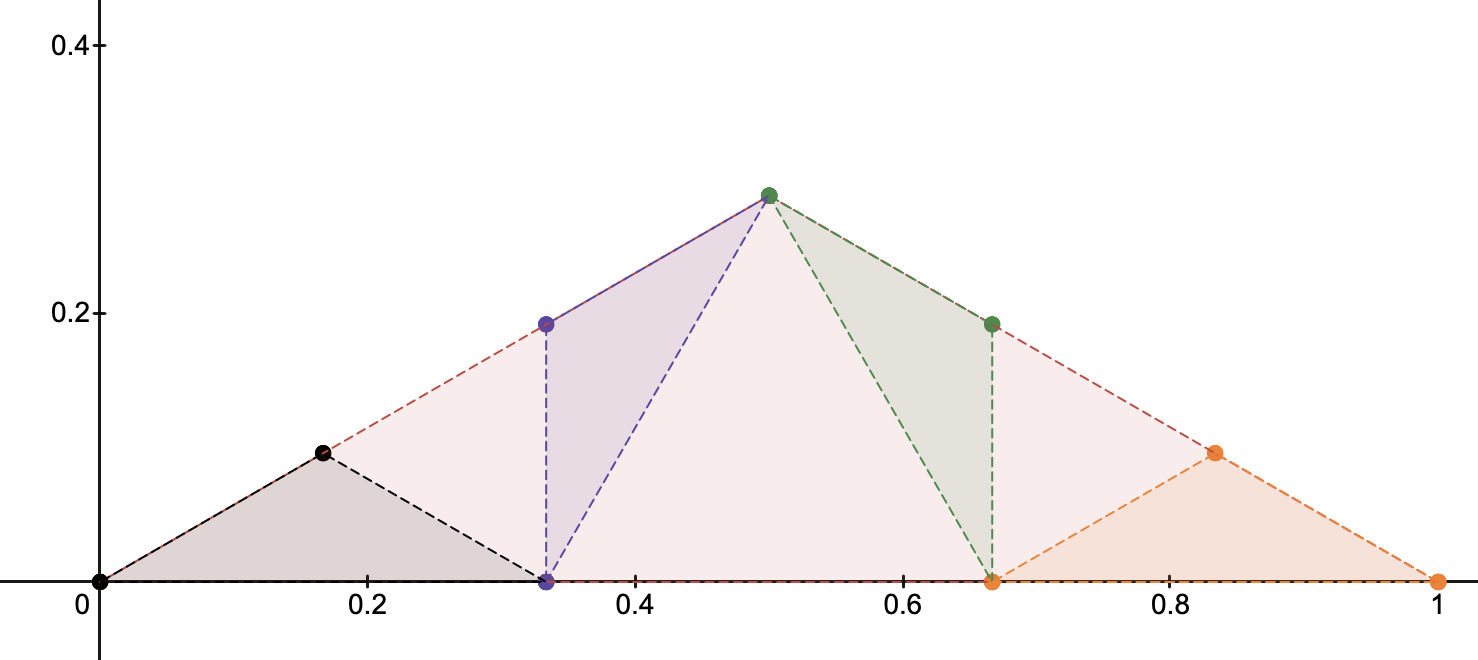
\includegraphics[scale=0.5]{solutions/section-4-1/diag-4-1-2.png}
\end{center}

The contraction ratios are \(c_1 = c_2 = c_3 = c_4 = \frac{1}{3}\) from the definition of a Koch curve.

Therefore, solving
\[
\sum_{i = 1}^{4} \frac{1}{3^s} = 1 \iff 4 = 3^s \iff s = \frac{\log 4}{\log 3},
\]
which means the Hausdorff dimension of the Koch curve is \(\frac{\log 4}{\log 3}\).
\newpage

\section{Problem 4.1.3}
\textit{Proof:} B.W.O.C. assume the Cantor Set \(C\) was countable. By definition of a countable set, we could list the points as \(\{a_i\}_{i=1}^{+\infty}\). Recall that for \(s,\delta > 0\), 

\[\h_\delta^s (C) = \inf \left\{\sum_i |U_i|^s : \{U_i\}_i \text{ is a } \delta\text{-cover of } C \right\}.\]

Consider the cover \(\{A_i\}_i(\epsilon)\) for \(\epsilon > 0\), where \(A_i\) is the open interval of size \(\frac{\epsilon}{2^i}\) centered at \(a_i\), i.e., \(A_i = B_{a_i} \left(\frac{\epsilon}{2^i}\right)\). Since each point has an open interval covering it, this is clearly a cover of \(a_i\); and we can make the first set have diameter \(|A_1| < \delta\) by taking \(\epsilon\) to be arbitrarily small, so the it satisfies the condition, and since the set sizes monotonically decrease the rest of them also satisfy the condition. Thus the cover is a \(\delta\)-cover, and therefore
\begin{align*} 
 \h_\delta^s (C) &\leq \sum_{i=0}^\infty \left(\frac{\epsilon}{2^n}\right)^s \\
 &= \epsilon^s \sum_{i=0}^{\infty} (2^{-s})^n \\
 &= \frac{\epsilon^s}{1-2^{-s}}.
\end{align*}
Since \(s > 0\), this converges, and taking \(\epsilon\) arbitrarily small we can make this arbitrarily close to 0. This is true for each \(\delta\), so \(\h^s(C) \leq 0\). By 2.1.4.1, \(\h^s(C) \geq 0\), so \(\h^s = 0\). Hence the Hausdorff dimension of \(C\) is \(\leq s\) for all \(s > 0\). But taking \(s \ll \frac{\log(2)}{\log(3)}\), we know that the Hausdorff dimension of \(C\) \( \ll \frac{\log(2)}{\log(3)}\). However by Theorem 4.1.2 \(\frac{\log(2)}{\log(3)}\) was the unique Hausdorff dimension so this leads to a contradiction, and \(C\) cannot be countable.
\newpage

\section{Problem 4.1.4}
\textit{Proof:} Please add the solution to solutions/section-4-1/q-4-1-4.tex.
\newpage

\section{Problem 4.1.5}
\textit{Proof:} Consider the IFS \((f_1, f_2)\) defined on \(\R \to \R\) as follows:
\begin{itemize}
    \item \(f_1(x) = \frac{2}{3}x\),
    \item \(f_2(x) = \frac{2}{3}x + \frac{1}{3}\).
\end{itemize}

Note that they have contraction ratios \(c_1 = c_2 = \frac{2}{3}\).

Notice that \(D = [0, 1]\) is an attractor of this IFS, since
\begin{align*}
f_1([0, 1]) &= \left[0, \frac{2}{3}\right],\\
f_2([0, 1]) &= \left[\frac{1}{3}, 1\right],
\end{align*}
and therefore \(f_1(D) \cup f_2(D) = [0, 1] = D\).

The Hausdorff dimension of \([0, 1]\) is \(s = 1\). This can be shown by considering the IFS \((g_1, g_2)\) on \(\R\):
\begin{itemize}
    \item \(g_1(x) = \frac{1}{2}x\),
    \item \(g_2(x) = \frac{1}{2} x + \frac{1}{2}\).
\end{itemize}

Both \(g_1\) and \(g_2\) have contraction ratios \(\frac{1}{2}\), and its is easy to see it satisfies the OSC by taking \((0, 1)\) as the open set, and we can see as well that \([0, 1]\) is the attractor. Therefore, the Hausdorff dimension of \([0, 1]\) \(s'\) must satisfy that \(2 \cdot \frac{1}{2}^s = 1\), which gives \(s = 1\).

However, if the OSC holds, then the dimension should also satisfy that
\[
\sum_{i = 1}^{2} \left(\frac{2}{3}\right)^s = 1,
\]
which is clearly not the case. Therefore, the OSC does not hold for this IFS.
\newpage

\section{Problem 4.2.1}
\textit{Proof:} Please add the solution to solutions/section-4-2/q-4-2-1.tex.
\newpage

\section{Problem 4.2.2}
\textit{Proof:} We alter slightly the definition of the natural measure. Specifically, we assign an uneven amount of measure on the left interval created and the right interval created each step. Let \(0 < p < 1\) such that \(p \cdot 3^s > 1\) where \(s = \log 2 / \log 3\), i.e., \(p > \frac{1}{2}\). Let the IFS of the Cantor set be \((f_1, f_2)\) where \(f_1(x) = \frac{1}{3}x\) and \(f_2(x) = \frac{1}{3} x + \frac{2}{3}\), and we denote \(f_{i_1, i_2, \ldots, i_m} (E)\) to be \(f_{i_1}(f_{i_2}(\ldots(f_{i_m}(E))))\), where each \(i_k \in \{1, 2\}\). Let \(t_1 = p, t_2 = 1 - p\), and define the measure \(\mu\) such that
\[
\mu\left(f_{i_1, i_2, \ldots, i_m} (C)\right) = \mu\left(f_{i_1, i_2, \ldots, i_m} ([0, 1]) \cap C\right) = \prod_{j = 1}^{m} t_{i_j} = t_{i_1} t_{i_2} \ldots t_{i_m}.
\]

This means every time a left interval is created, it takes up \(p\) of the measure of the original interval, with the right interval taking up \(1 - p\) of the measure.

Now, we can generalise this for any \(U \subset C\) simply using the similar concept as before, by approximating it with smaller and smaller intervals \(\cap C\):
\[
\mu(U) = \inf\left\{\sum_{i = 1}^{\mu(E_i)} : U \subset \bigcup_{i} E_i, E_i \text{ is an interval in the construction}\right\}.
\]

It is not difficult to see the non-negativity and the measure of the empty set being zero from the definition. The countable additivity is also true: consider disjoint Borel subsets \(\{E_i\}\) of \(C\), we will have \(\mu (\bigcup E_i) = \sum \mu(E_i)\) since the intervals are either disjoint or contains one-another (and we obviously don't want them to contain one-another to get closer to the \(\inf\) since simply removing the smaller one won't change the validity of the cover), and so they are disjoint, and so this holds.

Now consider \(\frac{\mu(U)}{|U|^s}\) for \(U = f_{1, 1, \ldots, 1}(C)\) where there are \(n\) 1s. It's not difficult to see that
\[
|U| = \left(\frac{1}{3}\right)^n,
\]
and that
\[
\mu(U) = p^n.
\]

Notice that
\[
\frac{\mu(U)}{|U|^s} = \frac{p^n}{3^{-sn}} = (2p)^n.
\]

Notice that this value decreases as \(p\) increases. For any \(\epsilon > 0\), we can find \(n\) that is sufficiently big enough such that \(|U| = 3^{-n} > \epsilon\), and for any \(c > 0\), we can further increase \(n\) to be big enough such that \(\mu(U) / |U|^s = (2p)^n > c\), since \(2p > 1\) and \((2p)^n\) is increasing with respect to \(n\). This means that for all \(c, \epsilon > 0\), we can find some \(U \subset C, |U| \leq \epsilon\), such that \(\mu (U) > c|U|^s\) for this measure \(\mu\) that we just constructed, as desired.
\newpage

\section{Problem 4.2.3}
\textit{Proof:} Please add the solution to solutions/section-4-2/q-4-2-3.tex.
\newpage

\section{Problem 4.2.4}
\textit{Proof:} Consider the set \(V = \left(-\frac{1}{4}, \frac{5}{4}\right) = \left(-\frac{3}{12}, \frac{15}{12}\right)\). For the IFS \((f_1, f_2)\) for the Cantor set \(C\), we have
\begin{align*}
    f_1(x) &= \frac{x}{3},\\
    f_2(x) &= \frac{x}{3} + \frac{2}{3}.
\end{align*}

Therefore, we have
\begin{align*}
    f_1(V) &= \left(-\frac{1}{12}, \frac{5}{12}\right),\\
    f_2(V) &= \left(\frac{9}{12}, \frac{13}{12}\right).
\end{align*}

Apparently \(f_1(V) \subset V, f_2(V) \subset V, f_1(V) \cap f_2(V) = \emptyset\). \(V \supset [0, 1] \supset C\) so not only does \(V\) satisfy the strong open set condition that \(C \cap V = C \neq \emptyset\), \(V\) also satisfies that \(V \supset C\) that it contains \(C\) completely.

For the Sierpinski Carpet, it is possible for \(V = (0, 1)^2\) to satisfy the SOSC. Recall that the IFS for the Sierpinski Carpet satisfies that

\begin{align*}
    g_1((x, y)) &= \left(\frac{x}{3}, \frac{y}{3}\right),\\
    g_2((x, y)) &= \left(\frac{x}{3}, \frac{y}{3} + \frac{1}{3}\right),\\
    g_3((x, y)) &= \left(\frac{x}{3}, \frac{y}{3} + \frac{2}{3}\right),\\
    g_4((x, y)) &= \left(\frac{x}{3} + \frac{1}{3}, \frac{y}{3}\right),\\
    g_5((x, y)) &= \left(\frac{x}{3} + \frac{1}{3}, \frac{y}{3} + \frac{2}{3}\right),\\
    g_6((x, y)) &= \left(\frac{x}{3} + \frac{2}{3}, \frac{y}{3}\right),\\
    g_7((x, y)) &= \left(\frac{x}{3} + \frac{2}{3}, \frac{y}{3} + \frac{1}{3}\right),\\
    g_8((x, y)) &= \left(\frac{x}{3} + \frac{2}{3}, \frac{y}{3} + \frac{2}{3}\right),\\
\end{align*}
and therefore
\begin{align*}
    g_1(V) &= \left(0, \frac{1}{3}\right) \times \left(0, \frac{1}{3}\right),\\
    g_2(V) &= \left(0, \frac{1}{3}\right) \times \left(\frac{1}{3}, \frac{2}{3}\right),\\
    g_3(V) &= \left(0, \frac{1}{3}\right) \times \left(\frac{2}{3}, 1\right),\\
    g_4(V) &= \left(\frac{1}{3}, \frac{2}{3}\right) \times \left(0, \frac{1}{3}\right),\\
    g_5(V) &= \left(\frac{1}{3}, \frac{2}{3}\right) \times \left(\frac{2}{3}, 1\right),\\
    g_6(V) &= \left(\frac{2}{3}, 1\right) \times \left(0, \frac{1}{3}\right),\\
    g_7(V) &= \left(\frac{2}{3}, 1\right) \times \left(\frac{1}{3}, \frac{2}{3}\right),\\
    g_8(V) &= \left(\frac{2}{3}, 1\right) \times \left(\frac{2}{3}, 1\right),\\
\end{align*}
and we can see they are pairwise disjoint and all subsets of \(V\). Furthermore, let \(g(E) = \bigcup_{i = 1}^{8} g_i(E)\), note that the point \(\left(\frac{1}{3}, \frac{1}{3}\right) \in V\), and also note that
\[
g_8((1, 1)) = (1, 1) \implies (1, 1) \in g^{(k)}([0, 1]^2),
\]
\[
g_1((1, 1)) = \left(\frac{1}{3}, \frac{1}{3}\right),
\]
and therefore
\[
\left(\frac{1}{3}, \frac{1}{3} \in g^{(k)}([0, 1]^2)\right),
\]
and therefore \(\left(\frac{1}{3}, \frac{1}{3}\right) \in \square\), the Sierpinski Carpet. But \(\left(\frac{1}{3}, \frac{1}{3}\right) \in V\) as well, so \(V \cap C \supset \left\{\left(\frac{1}{3}, \frac{1}{3}\right)\right\}\), and therefore \(V \cap C \neq \emptyset\).

However, it is impossible for such \(V \supset C\) to satisfy the SOSC. This is because if \(V \supset C\), then \((0, 1) \in V, (1, 1) \in V\). But notice
\[
g_4((0, 1)) = \left(\frac{1}{3}, \frac{1}{3}\right) = g_1((1, 1)),
\]
and therefore \(g_1(V) \cap g_4(V) \supset \left\{\left(\frac{1}{3}, \frac{1}{3}\right)\right\}\), and \(g_1(V) \cap g_4(V) \neq \emptyset\) which violates the pairwise disjoint condition of the OSC, hence the second part is impossible for the Sierpinski carpet.
\newpage

\section{Problem 4.2.5}
\textit{Proof:} Please add the solution to solutions/section-4-2/q-4-2-5.tex.
\newpage

\section{Problem 4.2.6}
\textit{Proof:} Please add the solution to solutions/section-4-2/q-4-2-6.tex.
\newpage

\section{Problem 5.0.1}
\textit{Proof:} Let \(s = \frac{\log 3}{\log 2}\). We restate some definitions first: let \(I_n = (i_1, i_2, \ldots, i_n) \in \{1, 2, 3\}^n\) where \(i_k \in \{1, 2, 3\}\) for each \(1 \leq k \leq n\), and define \(S_{I_n}(\Delta) = S_{i_1}(S_{i_2}(\ldots(S_{i_n}(\Delta))))\) where \(\Delta\) is the closed equilateral triangle with vertices \((0, 0), (1, 0)\) and \(\left(\frac{1}{2}, \frac{\sqrt{3}}{2}\right)\).

We define for \(E \subset \R^2\) that
\[
S(E) = \bigcup_{i = 1}^{3} S_i(E).
\]

\begin{itemize}
    \item \textbf{Upper Bound: \(\h^s(\sierpinski) \leq  1\).} Recall the definition that
    \[
    \h^s_\delta(\sierpinski) = \inf_{\{U_i\} \text{ is a }\delta\text{-cover of }\sierpinski} \sum_{i = 1}^{+\infty} |U_i|^s.
    \]

    We can first show that \(|\triangle| \geq 1\) since \(|(0, 0) - (1, 0)| = 1\) and \(|\triangle| \leq 1\) since \(\triangle \subset \overline{B_{(0, 0)} (1)}\). And therefore, we can see that
    \[
    \left|S_{I_n}(\triangle)\right| = \frac{1}{2^n}
    \]
    from the definition of a contraction immediately.

    By theorem 4.0.2, we can see that
    \[
        \sierpinski = \bigcap_{k = 0}^{+\infty} S^{(k)}(\Delta)
    \]
    since \(\sierpinski\) is the attractor of the IFS.

    Consider a certain \(k \in \Z, k \geq 0\), and it is not difficult to see from definition that
    \[
        S^{(k)} (\Delta) = \bigcup_{I_n \in \{1, 2, 3\}^n} S_{I_n} (\Delta)
    \]
    from the definition of \(S^{(k)}\). (This can be shown by induction on \(k\).)

    Therefore, we can see
    \[
        \sierpinski \subset \bigcup_{I_n \in \{1, 2, 3\}^n} S_{I_n} (\Delta),
    \]
    and therefore, \(\{S_{I_n} (\Delta)\}\) gives a \(\delta\)-cover for \(\sierpinski\), when \(\delta > \frac{1}{3^n} \iff 3^n > \frac{1}{\delta} \iff n > -\log_3(\delta)\).

    Also, notice that \(\# \{S_{I_n} (\Delta)\} = 3^n\).

    Therefore, for any \(0 < \delta < 1\), choose \(n = \floor{-\log_3(\delta)} + 1 \implies n > -\log_3(\delta)\), and therefore
    \begin{align*}
        \h^s_\delta(\sierpinski) &= \inf_{\{U_i\} \text{ is a }\delta\text{-cover of }\sierpinski} \sum_{i = 1}^{+\infty} |U_i|^s\\
        &\leq \sum_{i = 1}^{3^n} \left(\frac{1}{2^n}\right)^{s}\\
        &= 3^n \cdot \frac{1}{2^{\left(n \cdot \log_2(3)\right)}}\\
        &= 3^n \cdot \frac{1}{3^n}\\
        &= 1,
    \end{align*}
    and therefore
    \[
        \h^s(\sierpinski) = \lim_{\delta \to 0} \h^s_\delta(\sierpinski) \leq 1,
    \]
    which shows the upper bound as desired.

    \item We show that the IFS of the Sierpinski triangle satisfies the OCS. Consider the open set \(U\) which is the open triangle with vertices \((0, 0), (1, 0), \left(\frac{1}{2}, \frac{\sqrt{3}}{2}\right)\). We notice that
    \begin{align*}
        S_1(U) &\text{ is an open triangle with vertices } (0, 0), \left(\frac{1}{2}, 0\right), \left(\frac{1}{4}, \frac{\sqrt{3}}{4}\right),\\
        S_2(U) &\text{ is an open triangle with vertices } \left(\frac{1}{2}, 0\right), \left(1, 0\right), \left(\frac{3}{4}, \frac{\sqrt{3}}{4}\right),\\
        S_3(U) &\text{ is an open triangle with vertices } \left(\frac{1}{4}, \frac{\sqrt{3}}{4}\right), \left(\frac{3}{4}, \frac{\sqrt{3}}{4}\right), \left(\frac{1}{2}, \frac{\sqrt{3}}{2}\right),
    \end{align*}
    and therefore they are pairwise disjoint and are all subsets of \(U\). Therefore the IFS satisfies the open set condition.
    
    Now, we show that the natural measure on \(\sierpinski\) satisfies the hypothesis for the mass distribution principle, for \(\epsilon = 1\) and \(c = 6\).

    Consider some \(U \subset \sierpinski\) such that \(|U| < 1\). There must exist some \(k\) such that \(2 \cdot 2^{-(k+1)} \leq |U| < 2 \cdot 2^{-k}\) for some \(k \geq 1\). Then, \(U \subset \bigcup_{i = 1}^{6} \left(\Delta_{k}\right)_i \cap \sierpinski\), where \(\Delta_{t}\) is a triangle formed in the \(t\)'s iteration of the IFS. This means that \(U\) is in at most \(6\) triangles in the \(k\)-th iteration, as shown in the diagram below:

    \begin{center}
        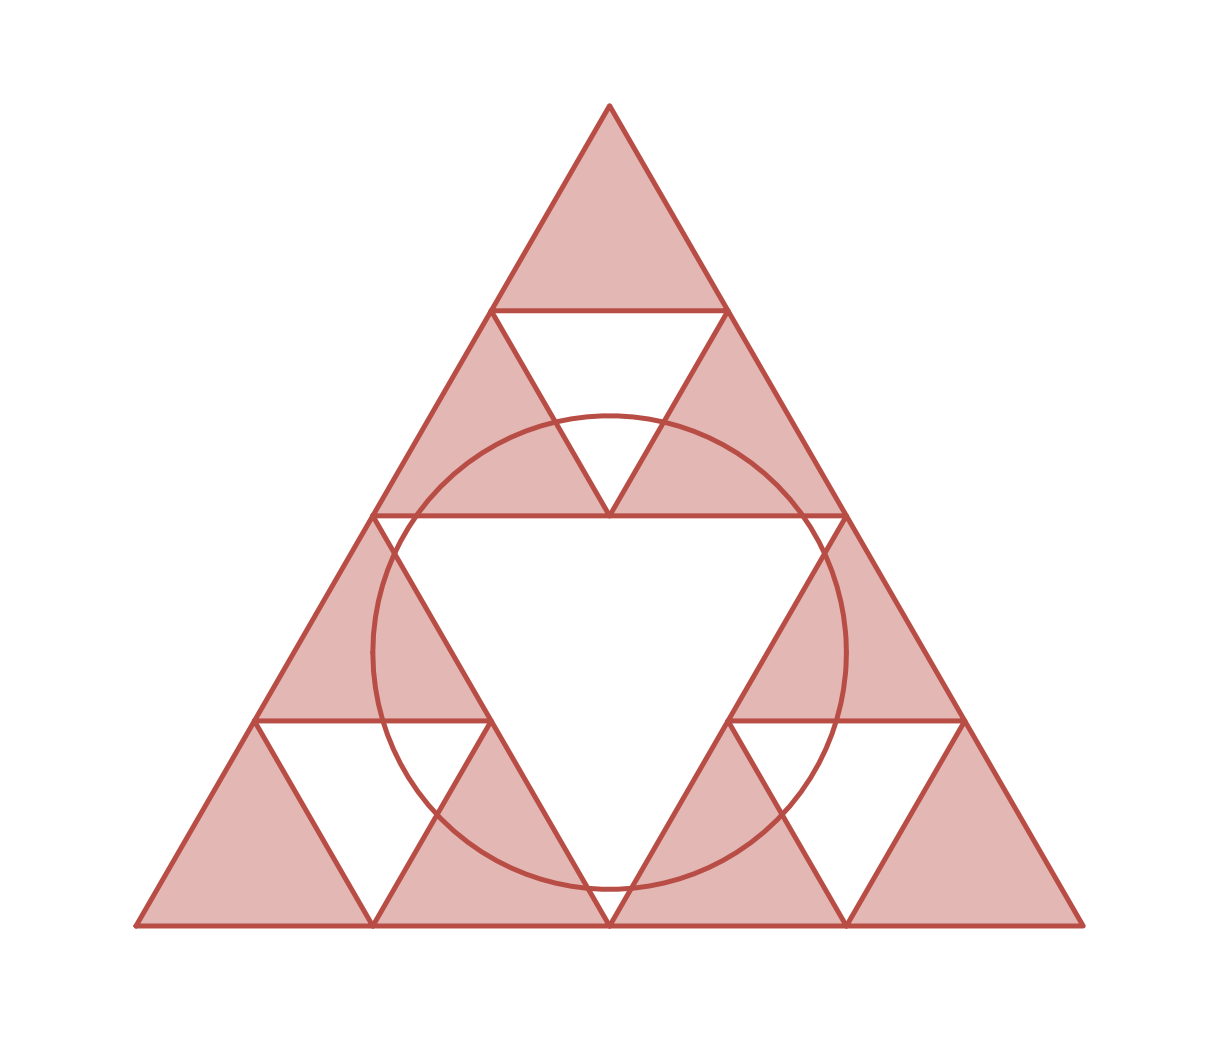
\includegraphics[scale=0.4]{solutions/section-5-0/diag-5-0-1.png}
    \end{center}
    
    Therefore we will have

    \begin{align*}
        \mu(U) & \leq 2 \cdot 3^{-k}\\
        &= 6 \cdot \left(2^{\log_2^3}\right)^{-(k+1)}\\
        &= 6 \cdot \left(2^{-(k+1)}\right)^{\log_2^3}\\
        &\leq 6 \cdot |U|^s.
    \end{align*}

    Notice that \(\mu(\sierpinski) = \mu(\Delta \cap \sierpinski) = \mu(S_{I_0} (\Delta) \cap \sierpinski) = 1\) and therefore,
    \[
    \h^s(\sierpinski) \geq \frac{\mu(\sierpinski)}{6} = \frac{1}{6}
    \]
    as desired.
\end{itemize}
\newpage

\section{Problem 5.0.2}
\textit{Proof:} Please add the solution to solutions/section-5-0/q-5-0-2.tex.
\newpage

\section{Problem 5.0.3}
\textit{Proof:} Please add the solution to solutions/section-5-0/q-5-0-3.tex.
\newpage

\section{Problem 5.0.4}
\textit{Proof:} \begin{center}
    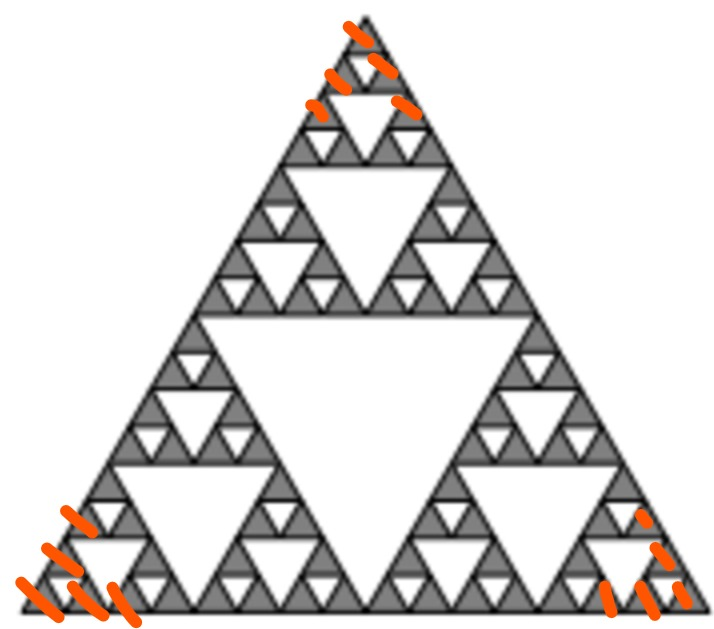
\includegraphics[scale=0.5]{solutions/section-5-0/diag-5-0-4.jpg}
\end{center}

This is one of the coverings of \(T_4\). The diameter is clearly \(\frac{13}{16}\) - as this is the distance between two opposite points in the figure. It also contains 66 out of 81 triangles - thus its value is \(\frac{\frac{13}{16}^s}{\frac{66}{81}}\) which is approximately \(0.8831093965\), notably less than \(0.9\). Hence \(a_4 \leq 0.8831093965 < 0.9\) so by theorem 5.0.2 the Hausdorff dimension is \(\leq 0.8831093965 < 0.9\), as required.
\newpage

\section{Problem 5.0.5}
\textit{Proof:} Recall the IFS \((m_1, m_2, \ldots, m_8)\) for the Minkowski Sausage \(M\) is:

\begin{align*}
    S_1((x, y)) &= \left(\frac{1}{4}x, \frac{1}{4}y\right),\\
    S_2((x, y)) &= \left(-\frac{1}{4}y + \frac{1}{4}, \frac{1}{4}x\right),\\
    S_3((x, y)) &= \left(\frac{1}{4}x + \frac{1}{4}, \frac{1}{4}y + \frac{1}{4}\right),\\
    S_4((x, y)) &= \left(\frac{1}{4}y + \frac{1}{2}, -\frac{1}{4}x + \frac{1}{4}\right),\\
    S_5((x, y)) &= \left(\frac{1}{4}y + \frac{1}{2}, -\frac{1}{4}x - \frac{1}{4}\right),\\
    S_6((x, y)) &= \left(\frac{1}{4}x + \frac{1}{2}, \frac{1}{4}y - \frac{1}{4}\right),\\
    S_7((x, y)) &= \left(-\frac{1}{4}y + \frac{3}{4}, \frac{1}{4}x - \frac{1}{4}\right),\\
    S_8((x, y)) &= \left(\frac{1}{4}x + \frac{3}{4}, \frac{1}{4}y\right).\\
\end{align*}

Notice this satisfies the OSC by considering a open square \(O\) with vertices at
\[(0, 0), (1, 0), \left(\frac{1}{2}, \frac{1}{2}\right), \left(\frac{1}{2}, -\frac{1}{2}\right),\] as shown in the following diagram.

\begin{center}
    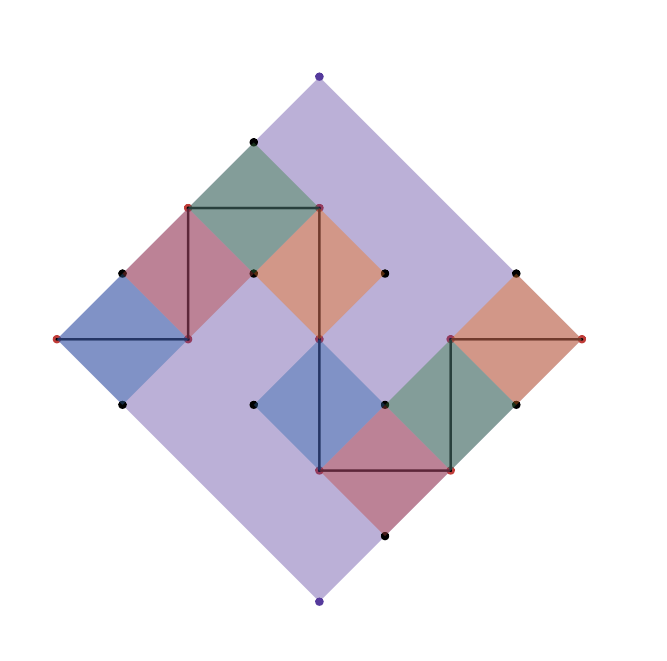
\includegraphics[scale=0.3]{solutions/section-5-0/diag-5-0-5-1.png}
\end{center}

Therefore, the dimension of \(M\), \(m\) must satisfy that
\[
8 \cdot \frac{1}{4^m} = 1 \iff m = \frac{3}{2} = 1.5,
\]
by theorem 4.1.2

Let \(M_0 = [0, 1]\) the closed interval. Let \(I_n = (i_1, i_2, \ldots, i_n)\) be a list with each \(i_k \in \{1, 2, \ldots, 8\}\), and set
\[
S_{I_n}(M_0) = S_{i_1}\left(S_{i_2}\left(\ldots\left(S_{i_n}(M_0)\right)\right)\right),
\]

Define the natural measure as
\[
\mu(S_{I_n}(M_0) \cap M) = \left(\frac{1}{4}\right)^{mn} = 8^{-n}.
\]

Let \(\mu\) be the natural measure on \(M\), the Minkowski sausage. Define
\[
\mathcal{M}_n = \{S_{I_n}(M_0) : I_n \in \{1, 2, \ldots, 8\}^n\}
\]
be the collection of all \(8^n\) scaling of size \(4^{-n}\) of the Minkowski Sausage, and let \(\{E_i\}_i \subset \mathcal{M}_n\) be a non-empty collection of those iterations of the scaling, define
\[
b_n = \min_{\{E_i\}_i \subset \mathcal{M}_n} \left\{\frac{|\bigcup_i E_i|^m}{\mu(\bigcup_i E_i)}\right\}.
\]

\textbf{Claim.} \(\h^m(M) \leq b_n\).

\textit{Proof.} We first show \(\h_\delta^m(M) \leq b_n\) for \(\h_1^m(M)\).

Since \(b_n\) is a minimum of some finite number of possibilities (subsets of the finite set \(\mathcal{M}_n\)), so there must be a collection of set \(U\) with \(\#U = k\) that gives the minimum of \(b_n\). Let \(\mathcal{U} = \bigcup_{E_i \in U} E_i\), the union of the elements in the collection \(U\).

In the case where \(\mathcal{U} = M\) is the Minkowski Sausage, then we see that this must be a cover of the Minkowski Sausage. In this case,
\[
b_n = \frac{|M|^m}{\mu(M)} \geq \frac{1^m}{1} = 1,
\]
since notice that the Minkowski Sausage contains the points \((0, 0)\) and \((1, 0)\) and they are distance of 1 apart, and noticing that \(S_{I_0} (M) = M\) so \(\mu(M) = 1\) naturally.

On the other hand, notice that \(\h_{1}^m(M) \leq 1^m = 1\) since the set containing the closed square with vertices at \((0, 0), (1, 0), \left(\frac{1}{2}, \frac{1}{2}\right)\) covers \(M\) and has diameter \(1\), and therefore from the definition, \(\h_{1}^m(M) \leq 1\) as desired. Therefore, \(\h_1^m(M) \leq 1 \leq b_n\) and satisfies the claim as desired.

Otherwise, let \(V = \mathcal{M}_n \setminus U\), all sets that are not contained in the collection \(U\). \(\# V = 8^n - k\). If for some \(S_{I_n} (M) = E_{m}' \in V\) that is not in \(U\), we scale down of these, and place it in \(V\) in the sense \(\mathcal{M}_{2n}\), the \(2n\)-th level of the construction of \(M\). If \(U\) is scaled down to \(U'\) and \(\mathcal{U}' = \bigcup_{E_i \in U} E_i\), we will see \(|\mathcal{U}'| = 4^{-n}|\mathcal{U}|\). Therefore, there will be \(8^n - k\) copies of these \(U'\)(s), one each for each element in \(\mathcal{M}_n\) that \(U\) does not hit. However this still does not cover \(M\) (since there are still missing pieces in each of parts of \(V\)), so we repeatedly create \(U''\), \(U'''\), etc.

Therefore, we cover \(M\) using 1 copy of \(\mathcal{U}\), \((8^n - k)\) copies of \(\mathcal{U}'\), \((8^n - k)^2\) copies of \(\mathcal{U}''\), and so on. Therefore,
\begin{align*}
    \h_1^m(M) &\leq \sum_{i = 0}^{+\infty} (8^n - k)^i |\mathcal{U}^{(i)}|^m\\
    &= \sum_{i = 0}^{+\infty} (8^n - k)^i (4^{-in} |\mathcal{U}|)^m\\
    &= |\mathcal{U}|^m \sum_{i = 0}^{+\infty} \left(\frac{8^n - k}{8^n}\right)i\\
    &= \frac{|\mathcal{U}|^s}{1 - \frac{8^n - k}{8^n}}\\
    &= \frac{|\mathcal{U}|^s}{\frac{k}{8^n}}\\
    &= \frac{|\mathcal{U}|^s}{\mu(\mathcal{U})}\\
    &= b_n,
\end{align*}
the first inequality sign arising due to definition, the second due to what we just show, the third by sum properties, the fourth by geometric series, the fifth by trivial algebra, the sixth by the definition of \(\mu(\mathcal{U})\) and that \(\mathcal{U}\) being the union of \(k\) copies of the \(n\)th iteration of the Minkowski Sausage which only share at most points which has dimension \(0\) so zero \(m\)-dimension measure, the seventh equal sign simply by definition of \(b_n\).

Now, we move on to \(\delta < 1\), and there must exist some \(t \in \N\) such that \(4^{-t} < \delta\). Therefore, instead with starting the cover \(U\) states in the previous part, we simply start with \(8^t\) copies of \(U\) scaled down by \(4^{-t}\), one at each level \(t\) iteration of \(M\). Then we simply preform the same process for each scaled down copies of \(U\), and at each stage we get \(8^n\) extra copies of \(U^{(n)}\), with a diameter scaled by \(4^{-n}\), and therefore
\begin{align*}
    \h_{\delta}^m(M) &\leq 8^t \sum_{i = 0}^{+\infty} (8^n - k)^i (4^{-t} |\mathcal{U}^{(n)}|)^m\\
    &= 8^t \cdot 4^{-t \cdot \frac{3}{2}} \sum_{i = 0}^{+\infty} (8^n - k)^i (|\mathcal{U}^{(n)}|)^s\\
    &= \sum_{i = 0}^{+\infty} (8^n - k)^i (|\mathcal{U}^{(n)}|)^s\\
    &= b_n
\end{align*}
similar to earlier. The largest size we used in this cover is \(4^{-t} < \delta\) is valid. Therefore, if we take the limit \(\delta \to \infty\), we will have
\[
\h^m(M) \leq b_n.
\]

Now consider the bounds of \(b_n\) when \(n = 2\). Consider the following diagram of the second iteration of \(M\), i.e., \(\mathcal{M}_2\).

\begin{center}
    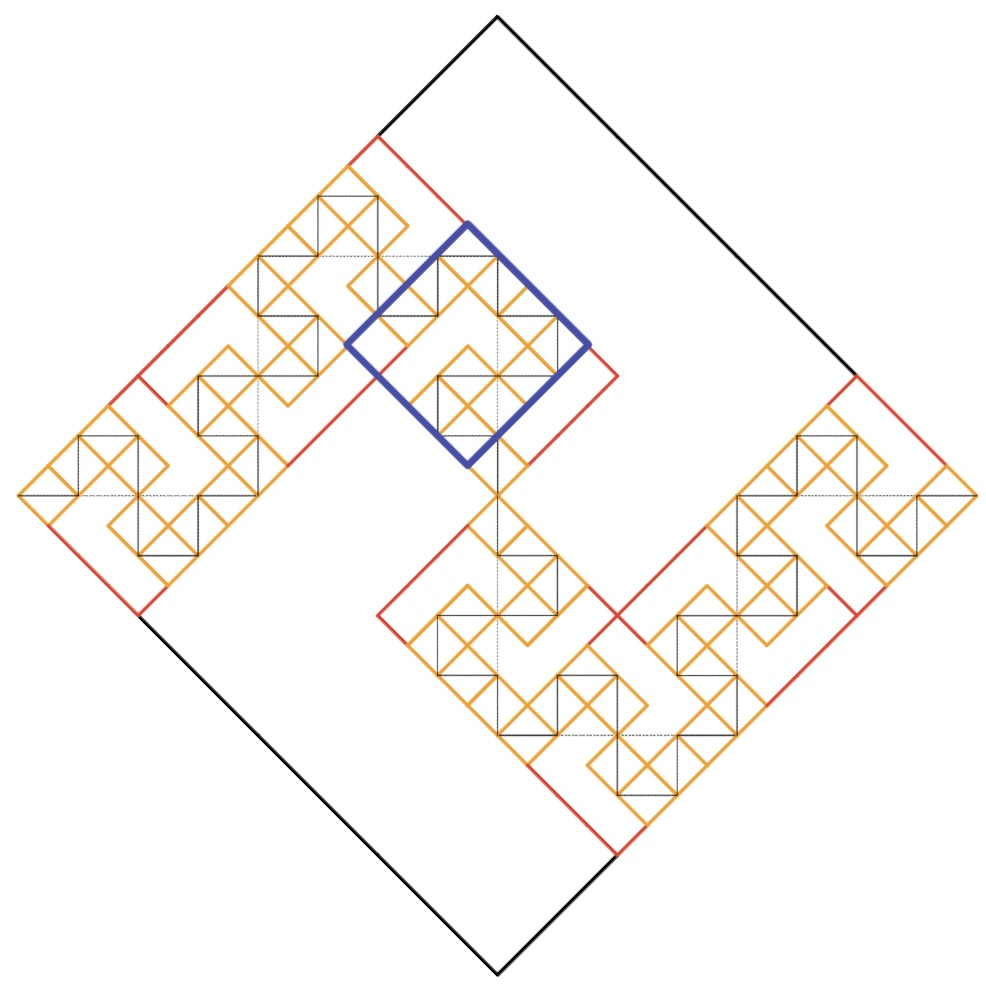
\includegraphics[scale=0.3]{solutions/section-5-0/diag-5-0-5-2.jpg}
\end{center}

It is worth mentioning why this diagram makes sense and what are the different elements of the diagram. First, note that \(M_0 = [0, 1] \subset\) the black square, which is a closed square with vertices at \((0, 0), (1, 0), \left(\frac{1}{2}, \frac{1}{2}\right), \left(\frac{1}{2}, -\frac{1}{2}\right)\). The first iteration of the black square is the eight red squares, which are all subsets of the black square. Therefore, the Minkowski Sausage \(M \subset\) the black square, and the first iteration of the Minkowski Sausage, elements in the set \(\mathcal{M}_1\), are each contained in one of the red squares. The first iteration of the red squares (the second iteration of the black square) are the orange squares, and elements in the set \(\mathcal{M}_2\) are each contained in one of the orange squares.

Now, we investigate the 10 orange squares marked in blue, and let our \(U \subset \mathcal{M}_2\) be the set of the 10 elements of \(\mathcal{M}_2\) contained in the 10 orange squares. We know that \(|\mathcal{U}| \leq |\text{blue square}| = \frac{1}{4}\) since \(\mathcal{U} \subset \) blue square.

Furthermore, each element in \(U\) has measure \(8^{-2} = \frac{1}{64}\), and therefore since there are 10 elements in \(U\), \(\mathcal{U}\) will have measure \(\frac{10}{64} = \frac{5}{32}\). Therefore,
\begin{align*}
    \h^m(M) &\leq b_2\\
    &\leq \frac{|\mathcal{U}|^m}{\mu(\mathcal{U})}\\
    &\leq \frac{4^{-\frac{3}{2}}}{\frac{5}{32}}\\
    &= \frac{\frac{1}{8}}{\frac{5}{32}}\\
    &= \frac{4}{5}\\
    &= 0.8
\end{align*}
as desired.
\newpage

\section{Problem 5.0.6}
\textit{Proof:} We show that \(a_3\) equals \(0.910411\) -- precisely
\[\frac{7^{\frac{\log(3)}{\log(2)}}}{24}.\]

This is done using this program, which brute-forces every combination of triangles to make the cover, finds the diameter, and computes the value of \(a_3\). Then it finds the minimum out of all these values and prints it out. This is extremely naive and would not work for \(a_4\).


\begin{verbatim}
#include <cmath>
#include <vector>
#include <set>
#include <tuple>
#include <algorithm>
#include <iostream>
#include <limits>

using namespace std;
using Point = pair<double, double>;
using Triangle = vector<Point>;

double root3 = sqrt(3.0);
double s = log(3.0) / log(2.0);

Point div(const Point& pt, double x) {
    return {pt.first / x, pt.second / x};
}

Point add(const Point& pt1, const Point& pt2) {
    return {pt1.first + pt2.first, pt1.second + pt2.second};
}

Point f0(const Point& pt) {
    return div(pt, 2.0);
}

Point f1(const Point& pt) {
    return add({0.5, 0.0}, div(pt, 2.0));
}

Point f2(const Point& pt) {
    return add({0.25, root3 / 4.0}, div(pt, 2.0));
}

using Func = Point (*)(const Point&);

vector<Func> funcs = {f0, f1, f2};

Triangle f(int n, const Triangle& tri) {
    Triangle result;
    for (const auto& pt : tri) {
        result.push_back(funcs[n](pt));
    }
    return result;
}

vector<Triangle> nexttri(const vector<Triangle>& tri) {
    vector<Triangle> tri1;
    for (const auto& t : tri) {
        for (int i = 0; i < 3; ++i) {
            tri1.push_back(f(i, t));
        }
    }
    return tri1;
}

set<Point> nextpts(const set<Point>& pts) {
    set<Point> pts1;
    for (const auto& pt : pts) {
        for (int i = 0; i < 3; ++i) {
            pts1.insert(funcs[i](pt));
        }
    }
    return pts1;
}

double dist(const Point& pt1, const Point& pt2) {
    return sqrt(pow(pt1.first - pt2.first, 2)
            + pow(pt1.second - pt2.second, 2));
}

double diameter(const set<Point>& pts) {
    double diam = 0.0;
    for (const auto& pt1 : pts) {
        for (const auto& pt2 : pts) {
            diam = max(diam, dist(pt1, pt2));
        }
    }
    return diam;
}

int main() {
    vector<Triangle> tri0 = {{{{0, 0}, {1, 0}, {0.5, root3 / 2}}}};
    set<Point> pts0 = {{0, 0}, {1, 0}, {0.5, root3 / 2}};

    auto tri1 = nexttri(tri0);
    auto pts1 = nextpts(pts0);
    int N = 3;

    for (int i=0;i<N-1;++i){
        tri1 = nexttri(tri1);
        pts1 = nextpts(pts1);
    }



    double mina = numeric_limits<double>::max();

    size_t numTriangles = tri1.size();

    double dd = -1, nn = -1; // store exact values
    for (size_t i = 1; i < (1u << numTriangles); ++i) {
        
        vector<Triangle> tri;
        set<Point> pts;

        for (size_t j = 0; j < numTriangles; ++j) {
            if (i & (1u << j)) {
                tri.push_back(tri1[j]);
                for (const auto& pt : tri1[j]) {
                    pts.insert(pt);
                }
            }
        }

        double d = diameter(pts);
        double n = static_cast<double>(tri.size());
        double a = pow(d, s) / (n / pow(3.0, N));
        if (a < mina) {
            mina = a;
            dd = d;
            nn = n;
        }
    }

    cout << mina << endl;
    cout << dd << " " << nn << endl;
    return 0;
}
\end{verbatim}

\newpage

\section{Problem 5.0.7}
\textit{Proof:} Please add the solution to solutions/section-5-0/q-5-0-7.tex.
\newpage
\end{document}

